% Options for packages loaded elsewhere
\PassOptionsToPackage{unicode}{hyperref}
\PassOptionsToPackage{hyphens}{url}
%
\documentclass[
]{book}
\usepackage{lmodern}
\usepackage{amssymb,amsmath}
\usepackage{ifxetex,ifluatex}
\ifnum 0\ifxetex 1\fi\ifluatex 1\fi=0 % if pdftex
  \usepackage[T1]{fontenc}
  \usepackage[utf8]{inputenc}
  \usepackage{textcomp} % provide euro and other symbols
\else % if luatex or xetex
  \usepackage{unicode-math}
  \defaultfontfeatures{Scale=MatchLowercase}
  \defaultfontfeatures[\rmfamily]{Ligatures=TeX,Scale=1}
\fi
% Use upquote if available, for straight quotes in verbatim environments
\IfFileExists{upquote.sty}{\usepackage{upquote}}{}
\IfFileExists{microtype.sty}{% use microtype if available
  \usepackage[]{microtype}
  \UseMicrotypeSet[protrusion]{basicmath} % disable protrusion for tt fonts
}{}
\makeatletter
\@ifundefined{KOMAClassName}{% if non-KOMA class
  \IfFileExists{parskip.sty}{%
    \usepackage{parskip}
  }{% else
    \setlength{\parindent}{0pt}
    \setlength{\parskip}{6pt plus 2pt minus 1pt}}
}{% if KOMA class
  \KOMAoptions{parskip=half}}
\makeatother
\usepackage{xcolor}
\IfFileExists{xurl.sty}{\usepackage{xurl}}{} % add URL line breaks if available
\IfFileExists{bookmark.sty}{\usepackage{bookmark}}{\usepackage{hyperref}}
\hypersetup{
  pdftitle={An Introduction to Generalized Linear Models},
  pdfauthor={Emma Grossman, Leah Marcus, Emily Palmer, Katherine Pulham, Andrew Rumments},
  hidelinks,
  pdfcreator={LaTeX via pandoc}}
\urlstyle{same} % disable monospaced font for URLs
\usepackage{color}
\usepackage{fancyvrb}
\newcommand{\VerbBar}{|}
\newcommand{\VERB}{\Verb[commandchars=\\\{\}]}
\DefineVerbatimEnvironment{Highlighting}{Verbatim}{commandchars=\\\{\}}
% Add ',fontsize=\small' for more characters per line
\usepackage{framed}
\definecolor{shadecolor}{RGB}{248,248,248}
\newenvironment{Shaded}{\begin{snugshade}}{\end{snugshade}}
\newcommand{\AlertTok}[1]{\textcolor[rgb]{0.94,0.16,0.16}{#1}}
\newcommand{\AnnotationTok}[1]{\textcolor[rgb]{0.56,0.35,0.01}{\textbf{\textit{#1}}}}
\newcommand{\AttributeTok}[1]{\textcolor[rgb]{0.77,0.63,0.00}{#1}}
\newcommand{\BaseNTok}[1]{\textcolor[rgb]{0.00,0.00,0.81}{#1}}
\newcommand{\BuiltInTok}[1]{#1}
\newcommand{\CharTok}[1]{\textcolor[rgb]{0.31,0.60,0.02}{#1}}
\newcommand{\CommentTok}[1]{\textcolor[rgb]{0.56,0.35,0.01}{\textit{#1}}}
\newcommand{\CommentVarTok}[1]{\textcolor[rgb]{0.56,0.35,0.01}{\textbf{\textit{#1}}}}
\newcommand{\ConstantTok}[1]{\textcolor[rgb]{0.00,0.00,0.00}{#1}}
\newcommand{\ControlFlowTok}[1]{\textcolor[rgb]{0.13,0.29,0.53}{\textbf{#1}}}
\newcommand{\DataTypeTok}[1]{\textcolor[rgb]{0.13,0.29,0.53}{#1}}
\newcommand{\DecValTok}[1]{\textcolor[rgb]{0.00,0.00,0.81}{#1}}
\newcommand{\DocumentationTok}[1]{\textcolor[rgb]{0.56,0.35,0.01}{\textbf{\textit{#1}}}}
\newcommand{\ErrorTok}[1]{\textcolor[rgb]{0.64,0.00,0.00}{\textbf{#1}}}
\newcommand{\ExtensionTok}[1]{#1}
\newcommand{\FloatTok}[1]{\textcolor[rgb]{0.00,0.00,0.81}{#1}}
\newcommand{\FunctionTok}[1]{\textcolor[rgb]{0.00,0.00,0.00}{#1}}
\newcommand{\ImportTok}[1]{#1}
\newcommand{\InformationTok}[1]{\textcolor[rgb]{0.56,0.35,0.01}{\textbf{\textit{#1}}}}
\newcommand{\KeywordTok}[1]{\textcolor[rgb]{0.13,0.29,0.53}{\textbf{#1}}}
\newcommand{\NormalTok}[1]{#1}
\newcommand{\OperatorTok}[1]{\textcolor[rgb]{0.81,0.36,0.00}{\textbf{#1}}}
\newcommand{\OtherTok}[1]{\textcolor[rgb]{0.56,0.35,0.01}{#1}}
\newcommand{\PreprocessorTok}[1]{\textcolor[rgb]{0.56,0.35,0.01}{\textit{#1}}}
\newcommand{\RegionMarkerTok}[1]{#1}
\newcommand{\SpecialCharTok}[1]{\textcolor[rgb]{0.00,0.00,0.00}{#1}}
\newcommand{\SpecialStringTok}[1]{\textcolor[rgb]{0.31,0.60,0.02}{#1}}
\newcommand{\StringTok}[1]{\textcolor[rgb]{0.31,0.60,0.02}{#1}}
\newcommand{\VariableTok}[1]{\textcolor[rgb]{0.00,0.00,0.00}{#1}}
\newcommand{\VerbatimStringTok}[1]{\textcolor[rgb]{0.31,0.60,0.02}{#1}}
\newcommand{\WarningTok}[1]{\textcolor[rgb]{0.56,0.35,0.01}{\textbf{\textit{#1}}}}
\usepackage{longtable,booktabs}
% Correct order of tables after \paragraph or \subparagraph
\usepackage{etoolbox}
\makeatletter
\patchcmd\longtable{\par}{\if@noskipsec\mbox{}\fi\par}{}{}
\makeatother
% Allow footnotes in longtable head/foot
\IfFileExists{footnotehyper.sty}{\usepackage{footnotehyper}}{\usepackage{footnote}}
\makesavenoteenv{longtable}
\usepackage{graphicx}
\makeatletter
\def\maxwidth{\ifdim\Gin@nat@width>\linewidth\linewidth\else\Gin@nat@width\fi}
\def\maxheight{\ifdim\Gin@nat@height>\textheight\textheight\else\Gin@nat@height\fi}
\makeatother
% Scale images if necessary, so that they will not overflow the page
% margins by default, and it is still possible to overwrite the defaults
% using explicit options in \includegraphics[width, height, ...]{}
\setkeys{Gin}{width=\maxwidth,height=\maxheight,keepaspectratio}
% Set default figure placement to htbp
\makeatletter
\def\fps@figure{htbp}
\makeatother
\setlength{\emergencystretch}{3em} % prevent overfull lines
\providecommand{\tightlist}{%
  \setlength{\itemsep}{0pt}\setlength{\parskip}{0pt}}
\setcounter{secnumdepth}{5}
\usepackage{booktabs}
\usepackage{amssymb}
\usepackage[]{natbib}
\bibliographystyle{apalike}

\title{An Introduction to Generalized Linear Models}
\author{Emma Grossman, Leah Marcus, Emily Palmer, Katherine Pulham, Andrew Rumments}
\date{2021-03-10}

\begin{document}
\maketitle

{
\setcounter{tocdepth}{1}
\tableofcontents
}
\hypertarget{description-of-our-book}{%
\chapter{Description of our book}\label{description-of-our-book}}

Someone please update this.

We used \citep{dunn2018generalized}

(also cite data we use\ldots)

\hypertarget{intro}{%
\chapter{Introduction}\label{intro}}

\hypertarget{what-came-before---linear-models}{%
\section{What came before - Linear models}\label{what-came-before---linear-models}}

If you are reading this book, you might already be familiar with linear models. Given our data, if we make some key assumptions (see \ref{linear} ), we can perform inference or prediction by assuming that our response value forms a linear relationship with our explanatory variable (or variables).

The reasoning of linear models is often intuitive, if we make a scatterplot our data, and see this:

\begin{verbatim}
## -- Attaching packages --------------------------------------- tidyverse 1.3.0 --
\end{verbatim}

\begin{verbatim}
## v ggplot2 3.3.3     v purrr   0.3.4
## v tibble  3.0.6     v dplyr   1.0.4
## v tidyr   1.1.2     v stringr 1.4.0
## v readr   1.4.0     v forcats 0.5.1
\end{verbatim}

\begin{verbatim}
## -- Conflicts ------------------------------------------ tidyverse_conflicts() --
## x dplyr::filter() masks stats::filter()
## x dplyr::lag()    masks stats::lag()
\end{verbatim}

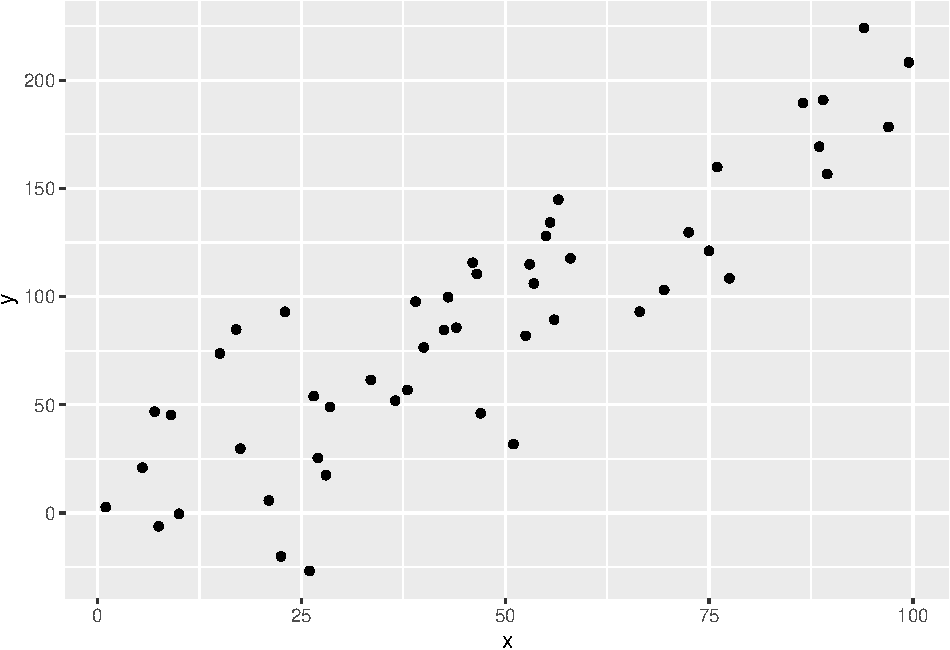
\includegraphics{Bookdown_files/figure-latex/unnamed-chunk-1-1.pdf}

we might want to fit a straight line through the cloud of points, i.e.~modeling the relationship linearly.

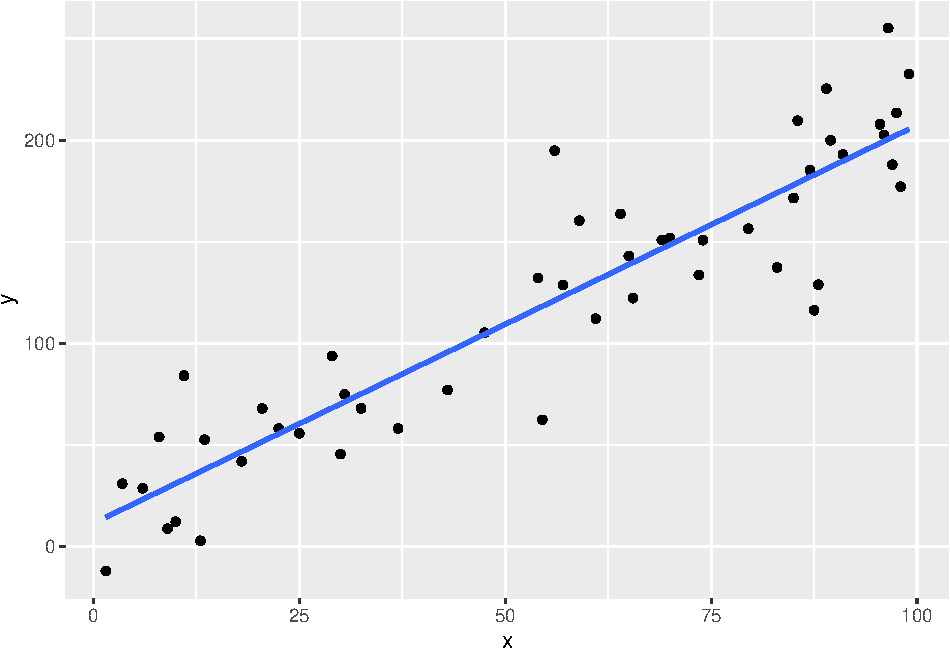
\includegraphics{Bookdown_files/figure-latex/lineplot-1.pdf}

To interpret this relationship and make predictions, we need to know the slope and intercept of this line. This is done by minimizing the least squares, which will be explored in chapter 3 @ref\{linear\}.

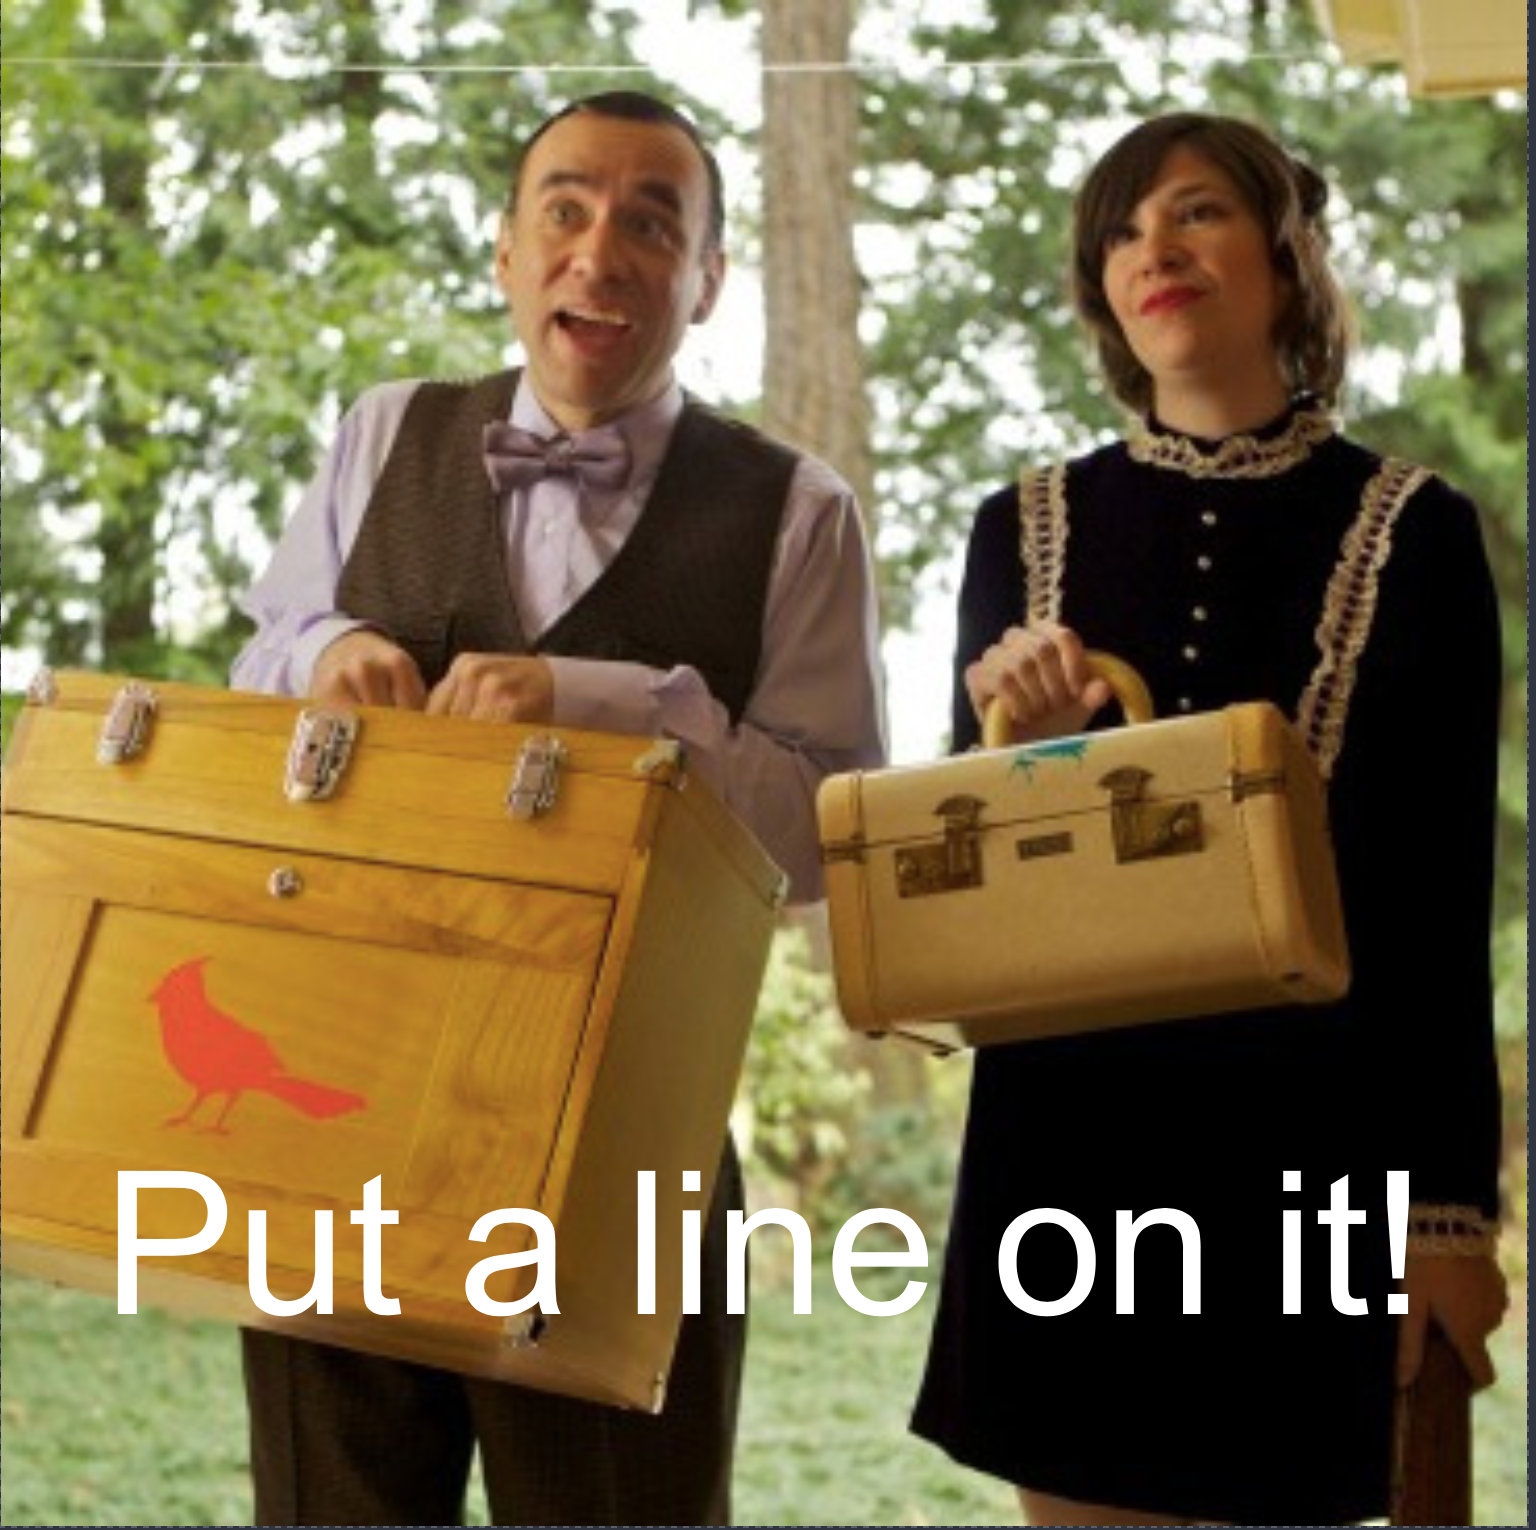
\includegraphics[width=0.5\textwidth,height=\textheight]{images/put_a_bird.png}

\hypertarget{some-definitions}{%
\section{Some definitions}\label{some-definitions}}

Predictor - the thing on the y-axis
Explanatory variable - the stuff on the x-axis. Note that we can have more than one (but won't plot it then), and then this becomes multivariate regression.

Something that is an estimated quantity will have a hat over it.
For example, we might assume that there is some `true' (but unknown) linear relationship between our explanatory variables and our predictor.

\[ y = \beta_0 + \beta_1 x\]

From our sample data, we use a linear model to make an estimate of \(\beta_0\) and \(\beta_1\),

so our estimate/best guess of this true model relationship is

\[ \hat y = \hat\beta_0 + \hat\beta_1 x\]
We of course want our \(\hat\beta_0\) and \(\hat\beta_1\) to be a `good' and `close' estimate of the unknown quantities \(\beta_0\) and \(\beta_1\). Ideas of what `good' and `close' mean will be covered in the next section.

\hypertarget{assumptions-of-linear-models}{%
\section{Assumptions of linear models}\label{assumptions-of-linear-models}}

A linear model might very well be a good model if our data look like \ref{fig:lineplot}. However, there are many cases where it might be inappropriate to use a linear model. To understand these cases, we first review the assumptions of linear models.

Linear models assume:

\begin{itemize}
\tightlist
\item
  The relationship between the explanatory variables and the response is linear
\item
  The samples are independent.
\item
  The errors are normally distributed with mean 0 and constant variance
\end{itemize}

We can write these assumptions down in notation as such.

\[y_i  = \beta_0 + \beta_1 x + \epsilon_i \]
where
\[ \epsilon_i \sim \text{iid } N(0,\sigma^2)\]
In words, this means that each
this means that the errors are independent and identically distributed by the normal distribution, with mean 0 and constant variance \(\sigma^2\) (notice how there is no subscript \(i\) for the variance)

If these assumptions hold, we then write our model as
\[ \hat y_i = \hat\beta_0 + \hat\beta_1 x_i\]

How can we tell when these assumptions are violated?

\begin{itemize}
\tightlist
\item
  Knowledge of the data.
\item
  Plots
\end{itemize}

\hypertarget{what-happens-when-we-break-the-assumptions-of-linear-models}{%
\section{What happens when we break the assumptions of linear models}\label{what-happens-when-we-break-the-assumptions-of-linear-models}}

Linear models are generally robust, and can be reasonable when assumptions are not exactly met. However, if we know assumptions are not met, and how they are not met, it is appropriate to use a more appropriate model for the data.

\hypertarget{random-and-systematic-component}{%
\section{Random and Systematic Component}\label{random-and-systematic-component}}

We will now analyze the assumptions for linear models and explore how we can generalize them. (and create generalized linear models!)

\[y_i  = \beta_0 + \beta_1 x + \epsilon_i \]
\[ \epsilon_i \sim \text{iid } N(0,\sigma^2)\]

We refer to the first equation as the Systematic Component, and the second equation as the Random Component.

A Generalized Regression Model has a systematic component:

\[ g(y_i) = \beta_0 + \beta_1 x + \epsilon_i\]
To generalized the systematic component, we use a link function \(g(y)\), so we now require some function of the response to be linearly related to our explanatory variables.

and a random component:

\[ \epsilon_i \sim \text{ iid } EDM(\phi) \]
In words, the errors are independently distributed according to some probability distribution in the Exponential Dispersion Family, which will be discussed in the next chapter. Normal, Binomial, and Poisson distributions all fall into this family.

We note that normal linear models fall exactly into this framework, where \(g(y_i) = y_i\) the identity function, and use the Normal distribution as our random component.

Deciding on what Random and Systematic component to use requires u

\hypertarget{random-and-systematic-components-for-binary-and-count-data}{%
\section{Random and Systematic components for Binary and Count data}\label{random-and-systematic-components-for-binary-and-count-data}}

The two most common cases of GRMs are those for Binary and Count data

For Binary data, the systemtatic component is, and the random component is: We call these types of GRMS logistic regression or \ldots{}

For Count data, the systematic component is, and the random component is. We call these types of GRMS

\hypertarget{parameter-estimation}{%
\section{Parameter estimation}\label{parameter-estimation}}

The last difference between linear models and generalized linear models is the way we estimate the parameters \(\beta\).

\hypertarget{conclusion}{%
\section{Conclusion}\label{conclusion}}

Linear models are not always the best tool for describing relationship in data. Luckily we can generalize the ideas and framework developed in linear models to hold for more general cases to create GLMs. Using a more general framework and more general assumptions allows us to build tools that will hold for all GRMs. The most notable of these that we will further explore are GRMs for binary data (ch4) and count data (ch5)

\hypertarget{examples}{%
\section{Examples}\label{examples}}

Perhaps some examples of data and students can tell what type of data it should be modeled by?

\hypertarget{how-are-glms-different}{%
\chapter{How are GLMs ``different''?}\label{how-are-glms-different}}

\hypertarget{introdution}{%
\section{Introdution}\label{introdution}}

So, we've talked about the issues that linear models can run into. The question now is how do we deal with these issues? What we're going to need to do is expand the type of model we're trying to fit. In linear regression we assumed two things: that the response variable \(Y_i\) is distributed normally, with constant variance \(\sigma^2\), and that the mean of the response variable is a linear combination of the explanatory variables. These two assumptions can be stated as

\begin{enumerate}
\def\labelenumi{\arabic{enumi}.}
\tightlist
\item
  \(Y_i \sim \mathcal{N}(\mu_i,\sigma^2)\)
\item
  \(\mu_i = \beta_0 + \beta_{1}X_{i,1}+...+\beta_{k}X_{i,k}\)
\end{enumerate}

In this chapter we're going to make our model more general by expanding these two assumptions. The first assumption, which we will call the random component, is going to change from \(Y\) being distributed normally to \(Y\) being distributed according to \emph{some probability family}. The second assumption is going to change from \(\mu_i\) directly equaling the linear predictor to \emph{some function} of \(\mu_i\) being equal to this linear predictor.

\hypertarget{assumptions-of-a-glm}{%
\section{Assumptions of a GLM}\label{assumptions-of-a-glm}}

GLMs are made up of two components: a random component, and a structural component. In general, what we're saying is that the response variable of interest is a random variable that follows a specific probability distribution (random component). This probability distribution is, in some way, related to a linear combination of the explanatory variables (systematic component). This linear combination of the explanatory variables is where the ``linear'' in ``generalized linear model'' comes from. In linear regression, which is a special case of the generalized linear model, the random component is that Y comes from a normal distribution: \(Y_i\sim N(\mu_i,\sigma^2)\) and the systematic component is that the mean is some linear combination of the explanatory variables: \(\mu_i=\beta_0+\beta_1X_{1i}+...+\beta_kX_{ki}\). With GLMs, our goal is to extend this framework so that we're not just limited to the normal distribution for the random component of our model, for reasons we discussed in the last chapter.

However, when we fit these models, we need to be sure of a couple of things. We need to ensure that for a linear combination of explanatory variables, we can identify which distribution the response variable comes from. We also need to ensure that the parameters of that distribution we're trying to fit are estimable. To ensure that we're able to properly fit these models, GLMs consider a specific kind of family of distributions for the random component: the Exponential Dispersion Model.

\hypertarget{framework}{%
\section{Framework}\label{framework}}

\hypertarget{exponential-dispersion-models}{%
\subsection{Exponential Dispersion models}\label{exponential-dispersion-models}}

An exponential dispersion model is a specific type of random variable, whose pdf follows a specific form:
\[
f_{Y}(y) = a(y,\phi)exp\left[\frac{y\theta - \kappa(\theta)}{\phi}   \right]
\]
in this form, \(\theta\) is called the \emph{canonical parameter}, and \(\phi\) is called the \emph{dispersion parameter}. For our purposes, the function \(a(y,\phi)\) is not of much interest, but it is needed to guarantee that \(f_Y(y)\) integrates to 1, and is therefore a valid probability density function. \(\kappa(\theta)\) is called the \emph{cumulant} function, and will be useful to us in estimation. Another term for an exponential dispersion model is to say that the family of random variables is an exponential family.

A surprising, and fortunate, number of families of distributions are exponential dispersion models. Notably, some of them are

\begin{itemize}
\tightlist
\item
  Normal random variables
\item
  Bernoulli random variables
\item
  Binomial random variables
\item
  Poisson random variables
\item
  Exponential random variables
\item
  Gamma random variables
\item
  Negative binomial random variables
\end{itemize}

We'll spare the details for most of these families, but to show the general idea for how we decide whether or not a family of random variables is an exponential dispersion model, we shall consider the poisson random variable.

\textbf{Example:} For a poisson random variable, the pmf is written as

\[
f_Y(y) = e^{-\lambda}\frac{\lambda^y}{y!}
\]

by applying the identity \(x=e^{log(x)}\) to the numerator, we see that this is equivalent to

\[
f_Y(y) =\frac{1}{y!} exp\left[-\lambda + y log(\lambda) \right] 
= \frac{1}{y!} exp\left[\frac{y log(\lambda) -\lambda}{1} \right] 
\]

and we see that the poisson random variable is an exponential dispersion model with dispersion parameter \(\phi = 1\), with canonical parameter \(\theta = log(\lambda)\) and with cumulant function \(\kappa(\theta) = \lambda = e^\theta\). Notice how we left out the \(\frac{1}{y!}\) term of the exponential because it was not needed to put the function into this important form. \(\Box\)

\hypertarget{properties-of-edms}{%
\subsection{Properties of EDMs}\label{properties-of-edms}}

Once we can get a probability distribution function into the exponential dispersion model form, we can connect this form to both the mean and variance of the random variable. The expected value (mean) of the random variable is simply the first derivative of the cumulant function with respect to the canonical parameter:
\[
E[Y] =\mu= \frac{d}{d\theta}\kappa(\theta)
\]
The cumulant function is also related to the variance of the random variable. The variance of the random variable is the dispersion parameter multiplied by the second derivative of the cumulant function with respect to the canonical parameter:
\[
var(Y) = \phi \frac{d^2}{d\theta^2} \kappa(\theta)
\]
The second part of this expression is an important quantity, called the variance function. Notice that it is equal to the first derivative of the expected value of Y as well:
\[
V(\mu) = \frac{d^2}{d\theta^2} \kappa(\theta) = \frac{d}{d\theta}\mu
\]
It is worth noting that, in addition to helping us estimate properties of \(Y\), the variance function uniquely determines the family of distributions (type of random variable) for a given EDM. For instance, following our previous example, since \(\kappa(theta) = e^{\theta}\), the variance function is \(V(\mu) = \frac{d^2}{d\theta^2} e^\theta = e^\theta = \lambda = \mu\). What this means is that \emph{any} EDM with variance function \(V(\mu) = \mu\) will be a poisson random variable.

\hypertarget{linking-the-edm-to-the-explanatory-data}{%
\subsection{Linking the EDM to the explanatory data}\label{linking-the-edm-to-the-explanatory-data}}

Recall, just for a second, the goal of constructing these models. We have a response variable, \(Y_i\), and a collection of explanatory variables \(X_1, X_2, X_3,...X_k\). We want to be able to look at a combination of the explanatory variables and draw some conclusions about \(Y\). Perhaps we want to predict Y with a point estimator. If we make this sort of prediction, it's also of interest to know how precise that estimate will be, so we may wish to find an interval estimate for the prediction as well. Ultimately, all of these things come from the distribution of \(Y\), so the thing that is of interest is to be able to know what the probability distribution of \(Y\) is given the input values of the \(X_i\)'s.

As stated before, the L in GLM stands for linear, and these explanatory variables are where that linearity comes into play. In GLMs, we're assuming that the quantity we'll use to predict the response variable \(Y\) is a linear combination of the explanatory data \(\beta_0+\beta_1X_{1}+...+\beta_kX_{k}\). We will call this quantity the linear predictor; a common shorthand way of writing it is to use the greek letter \(\eta = \beta_0+\beta_1X_{1}+...+\beta_kX_{k}\). In practice, we often have multiple repetitions of the explanatory variables, where \(Y_i\) is a random variable who's distribution is somehow linked to the covariates \(X_{1i}, X_{2i}, X_{3i},...X_{ki}\). In this case, we will denote the separate linear predictors as \(\eta_i = X_{1i}, X_{2i}, X_{3i},...X_{ki}\). Note that although the variables may change, the coefficients \(\beta_0, \; \beta_1, \; ... \; \beta_k\) are the same for every \(\eta_i\). These \(\beta\) coefficients are the thing we must estimate to fit our GLM.

The question remains of \emph{how} we connect \(\eta\) to the distribution of \(Y\). First, we have to suppose what kind of distribution \(Y\) is coming from (is it a poisson random variable? Binomial?) and then we need to find some function g() such that the expected value \(E[Y] = \mu\) is simply \(g(\mu) = \eta\). For this, we have to place a couple restrictions on g. First, g must be a strictly monotonic function (strictly increasing or strictly decreasing) from some subset of the real numbers onto the set of all values that \(\mu\) could be. We require the monotonicity to ensure that we don't have multiple separate means being linked to the same linear predictor. This function also has to be differentiable to make sure that the tools we use to estimate \(\mu\) don't break. In practice, these requirements don't come up very much, since typically there are a couple of link functions that get used for each family of probability densities.

One special link function for each EDM family is the \emph{canonical link function}. For an EDM family of distributions, the canonical link function is the function \(g(\mu)\) that satisfies \(\eta=\theta=g(\mu)\).

The canonical link function isn't the only valid link function. Take for example the binomial family of distributions, and let \(Y\sim Binom(n,p)\), for some known n.~Note that \(\mu = p\). In this case, the set of possible values of \(p\) is the unit interval \((0,1)\). The canonical link function for this family is the logit function:
\[
g(p) = log\left(\frac{p}{1-p}\right)
\]

However, there are a couple of other link functions that satisfy the required assumptions. Notably, we have the probit function:
\[
g(p)=\Phi^{-1}(p)
\]
which is just the inverse of the normal CDF \(\Phi\). In other words, \(\Phi^{-1}(p) = \xi\) where \(\xi\) is the real number that satisfies \(P(Z\leq\xi)=p\) with \(Z\) being a standard normal random variable (mean 0 and variance 1).

One more notable link function for the binomial family is complimentary log-log (or c-log-log) model. This link function is
\[
g(p) = log(-log(1-p))
\]

All three of these link functions map the real numbers to the unit interval (0,1). Note that since \(g(\mu)=\eta\), and since these link functions are invertible (guaranteed by differentiability and strict monotonicity), we can express this as \(\mu = g^{-1}(\eta)\). Often times this second form is a more intuitive way to think about how the linear predictors relate to the mean response.

It can be seen that all three of these link functions are sigmoid functions, but that they have slightly different properties:

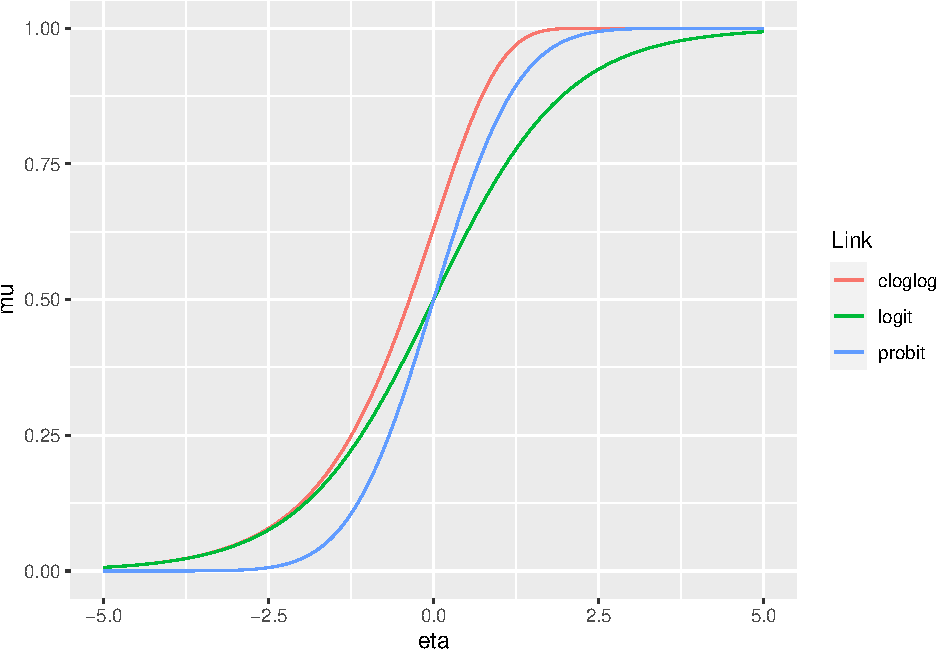
\includegraphics{Bookdown_files/figure-latex/unnamed-chunk-2-1.pdf}

The consequences of these differences will not be discussed here, this example exists purely to illustrate that an EDM family can have multiple distinct link functions. The consequenses of these varying link functions varies from family to family.

\hypertarget{formal-definition-of-a-glm}{%
\subsection{Formal definition of a GLM}\label{formal-definition-of-a-glm}}

Formally, a Generalized Linear Model is made of two components: the \emph{probability family} and the \emph{link function}. Given a set of data with response variable \(Y\) and explanatory variables \(X_1, ... X_k\), we wish to build a Generalized Linear Model. We assume that each \(Y_i\) follows a probability distribution from a given EDM family of distribution with mean \(\mu_i\) and dispersion parameter \(\phi\): \(\mu_i\) \(Y_i \sim EDM(\mu_i,\phi)\), where \(\mu_i\) is such that \(g(\mu_i) = \beta_0 + \beta_1X_{i,1} + ... \beta_kX_{i,k}\) for the link function \(g(\mu_i)\) and some vector of parameters \((\beta_0...\beta_k)\). We assume all of this is true, and then estimate the parameters \((\beta_0...\beta_k)\) using the data and maximum likelihood estimation algorithms. In this book, we will leave these estimation algorithms ``under the hood'' for brevity's sake, and focus on some common applications of these GLMs. Generally, to fit one of these models in R, you will need to know the family and the link function, as defined above.

\hypertarget{linear}{%
\chapter{Linear Models - Emma}\label{linear}}

\hypertarget{introduction}{%
\section{Introduction}\label{introduction}}

\begin{figure}
\centering
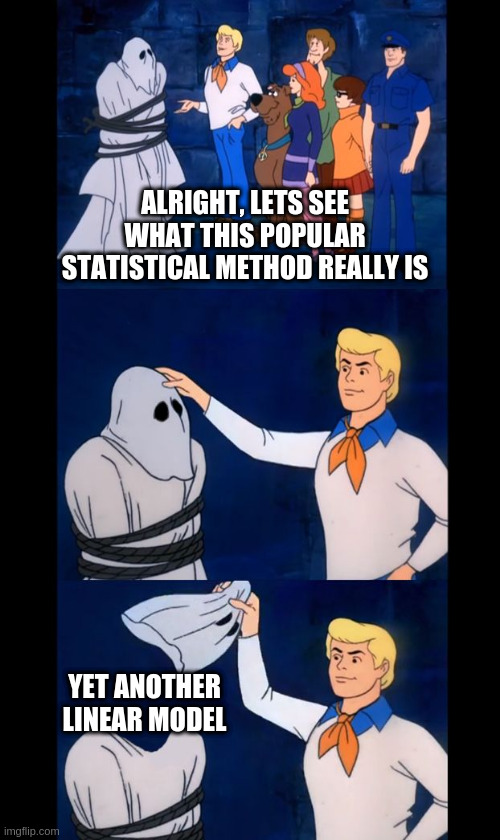
\includegraphics{images/scooby_doo_meme.jpg}
\caption{It's linear models all the way down. Posted on reddit in r/statisticsmemes by u/not\_really\_redditing.}
\end{figure}

At this point, you are likely familiar with linear regression. As discussed before, linear regression models are a special case of generalized regression model that we use when the data are normally distributed and have constant variance. We can think of linear regression models in the same terms we think of other regression models.

The two components of a regression model are the random component and the systematic component and for linear regression,

\[
\begin{cases}
  \text{var}[y_i] &= \sigma^2/w_i \\
  \mu_i &= \beta_0 + \sum_{j=1}^{p}\beta_jx_{ji}
\end{cases}
\]

where \(w_i\) are prior weights and \(w_i\) and \(\text{E}[y_i] = \mu_i\) are known.

When our linear regression has two \(\beta_j\) coefficients and the systematic compnent looks like \(\mu = \beta_0 + \beta_1x_1\), it is called \emph{simple linear regression}. If we have more than two \(\beta_j\) coefficients, our regression model is called \emph{multiple linear regression model} or \emph{multiple regression model}.

When all prior weights \(w_i\) are equal to one, our regression model is refered to as \emph{ordinary linear regression model} as opposed to when our prior weights \(w_i\) have values other than one and is called a \emph{weighted linear regression model}.

As mentioned before, the assumptions belonging to linear regression are:

\begin{enumerate}
\def\labelenumi{\arabic{enumi}.}
\tightlist
\item
  The relationship between \(\mu\) and each explanatory variable is \textbf{linear}.
\item
  The unexplained variation in our response is constant, otherwise known as \textbf{constant variance}.
\item
  Each datam is \textbf{independent} of all other data points.
\end{enumerate}

\hypertarget{logistic-regression---andrew}{%
\chapter{Logistic Regression - Andrew}\label{logistic-regression---andrew}}

We've asked you thus far to take our word regarding Generalized Linear Models (GLMs). In this chapter, we're going to take a look at a certain type of data that we know violates our assumptions: binomial data. Here we'll examine binomial data, see why ordinary least sqares falls apart, and consider some alternative methods (spoiler: it's going to be one of our generalized linear models).

\hypertarget{what-is-binomial-data}{%
\section{What is Binomial Data?}\label{what-is-binomial-data}}

\hypertarget{refresher-bernoulli-and-binomial}{%
\subsection{Refresher: Bernoulli and Binomial}\label{refresher-bernoulli-and-binomial}}

Bernoulli and Binomial random variables are some of the most important to consider, because they get at real the roots of representing the stata of the world. A Bernoulli random variable considers the simplest possible datum: whether something is, or it isn't. Numerically, we represent this as 1 or 0, just like computer data. And while I can use this to measure yes/no type data, such as ``does a person own at least one pet?'', an astute observer will realise the same idea can apply to a variety concepts including:

\begin{itemize}
\tightlist
\item
  success / failure,
\item
  wins / losses,
\item
  heads / tails,
\item
  exists / doesn't exist
\item
  has / doesn't have
\item
  is a member of a group of interest / is not a member
\item
  or even, was my prediction realized?
\end{itemize}

Often, whatever resulted in creating this single Bernoulli instance might be something that repeats. In fact, if we hope to apply statistics to it, there needs to be many instances. If we can assume a constant probability across all iterations of the events we're interested in, but want to ask questions about them in aggregate, that's Bernoulli Binomial (or just binomial for short). Some examples of questions that fall into binomial data would be:

\begin{itemize}
\tightlist
\item
  is this strategy effective (i.e.~does it affect the rates of success or failure across many trials?)
\item
  is this baseball team better than another (i.e.~do they win more games, not just a game?)
\item
  if I bet money on getting four heads in a row, what kind of odds makes that a good gamble?
\item
  if a mailcarrier is moving to a new route, if I know how many homes are \(\mu\)-probable to have an angry dog, what's the liklihood that mail carrier will encounter an angry dog?
\item
  if \(\mu\)-proportion of students have a medical condition I'm interested in, how many students will I need to talk to in order for it to be more likely than not I'll talk to x of them? Way more likely than not? Almost certain?
\item
  if my predictions are p-percent accurate, and the cost of failure is m dollars, is it worth spending more money for more accurate predictions?
\end{itemize}

Hopefully you'll agree with me that questions of this type are actually extremely common.

\hypertarget{representing-the-bernoulli-distribution}{%
\subsection{Representing the Bernoulli distribution}\label{representing-the-bernoulli-distribution}}

Different texts use different language, so it's to explain how we'll be talking about Bernoulli and binomial distributions here. First, here's the /Bernoulli distribution/ probability mass function.

\[\mathcal{P}(y;\mu)=\mu^{y}(1-\mu)^{1-\mu},\]
where \(y\in\{0, 1\}, 0\leq\mu\leq1\).

This might be a bit different than what you've seen before, so lets talk about each variable.

\begin{itemize}
\tightlist
\item
  \(\mathcal{P}\): (\(\texttt{\\mathcal\{P\}}\) in TeX) is the probability mass function of a certain outcome. \(\mathcal{P}(y;\mu)\) then is the probability of event \(y\) when the success has a probability of \(\mu\).
\item
  \(y\): is the number of successes. Since this is a single trial, it can only be 0 or 1 (described by the statement \(y\in\{0, 1\}\)).

  \begin{itemize}
  \tightlist
  \item
    Basically, it lets us choose whether we're predicting success or predicting failure all in one function.
  \item
    If we're interested in the liklihood of an event not occuring \(y=0\), \(\mu^0=1\), and the PMF simplifies to \(\mathcal{P(1,\mu)}=1-\mu\).
  \item
    Conversely, if we're interetsed in an event occuring, \(y-1\), \((1-\mu)^{(1-1)}=1\), and the PMF simplifies to \(\mathcal{P(1,\mu)}=\mu\).
  \end{itemize}
\item
  \(\mu\): (\(\texttt{\\mu}\) in TeX) is the probability of the event. But wait, isn't \(\mu\) the mean, and also the expected value? \textbf{Yes, exactly!} Those are all the same in this PMF, so we use the same variable. Because many text books need you to consider those ideas separatey so you can discover that relationship, you might see it recorded elsewhere as \(p\), but since demonstrating that is beyond our scope here, we'll use \(\mu\) to reduce complexity.
\item
  It complicates using the formula elsewhere, but we could rewrite this as:
  \[
  \mathcal{P}(y;\mu)=
  \begin{cases}
  \mu&\textrm{if }y=1\\
  1-\mu&\textrm{if }y=0\\
  \end{cases}, 0\leq\mu\leq1
  \]
\end{itemize}

\hypertarget{representing-the-binomial-distribution}{%
\subsection{Representing the binomial distribution}\label{representing-the-binomial-distribution}}

Intuitively, you likely recall that if \(P(\textrm{heads on one coinflip})=\frac{1}{2}\), then \[P(\textrm{heads twice on two coinflips})=P(\textrm{heads on one coinflip})^2=\frac{1}{2}\times\frac{1}{2}=\frac{1}{4}\]. However, just like the above PMF accounts for yes and no, our binomial PMF \(\mathcal{P}\) needs to account for yes and no, how many yesses we're looking for, and how many trials there are overall. So here, we'll use:

\[\mathcal{P}(y;\mu,m)=\binom{m}{my}\mu^y(1-\mu)^{m(1-y)}\]
where \(y={0, 1/m, 2/m, ..., 1}, m \textrm{ is a positive integer, and }0<\mu<1.\)

Like before, this format might be a bit different than what you may have seen elsewhere, so let's break it down.

\begin{itemize}
\tightlist
\item
  A reminder, \(\binom{n}{k}\), (written \texttt{\textbackslash{}texttt\{\textbackslash{}binom\{n\}\{k\}\}} in TeX) is a combination \(n\) choose \(k\). More detail \href{https://en.wikipedia.org/wiki/Combination}{here.}
\item
  \(\mathcal{P}\) (\(\texttt{\\mathcal\{P\}}\) in TeX) is the probability mass function (PMF) aka probability function. \(\mathcal{P}(y;\mu,m)\) then is the probability function of a binomial distribution for event \(y\) in the case of \(m\) Bernoulli trials with each trial having a probability of \(\mu\).
\item
  \(m\) here is simply the number of trials easy.
\item
  \(y\) here measures the \emph{proportion} of successes (and actually it really is above as well--I'll get to that in a moment).

  \begin{itemize}
  \tightlist
  \item
    For example, if there are 4 trials and we want to see two successes, \(y/m=2/4=0.5\)
  \item
    This interacts interestingly in the combinatorial component. That \(my\) will always equal the numerator of \(y\). In the previous example then, the \emph{choose} part of \(m\) choose \(my\) (aka \(\binom{m}{my}\)) will equal \(\binom{4}{2}\).
  \end{itemize}
\item
  If \(y=0\), \(\binom{m}{m0}=\binom{m}{0}=1\) (any choose 0, like any number raised to 0 equals 1). So, looking at this formula, if I want to know the odds of not getting any heads on four coin flips, then

  \begin{itemize}
  \tightlist
  \item
    \[\mathcal{P}(y;\mu,m)=\binom{m}{my}\mu^y(1-\mu)^{m(1-y)}=\binom{4}{4\times0}\mu^0(1-\mu)^{4(1-0)}=1\times1\times(1-\mu)^4\]
  \item
    So assuming a fair coin where \(\mu=\frac{1}{2}\), then \(\mathcal{P}(y;\mu,m)=\mu^4=(\frac{1}{2})^4=\frac{1}{16}\), which fits our expectations. Neat!
  \end{itemize}
\end{itemize}

\hypertarget{what-does-a-bunch-of-binomial-data-look-like-then}{%
\subsection{What does a bunch of binomial data look like then?}\label{what-does-a-bunch-of-binomial-data-look-like-then}}

\begin{Shaded}
\begin{Highlighting}[]
\NormalTok{possibilities \textless{}{-}}\StringTok{ }\KeywordTok{c}\NormalTok{(}\DecValTok{0}\NormalTok{,}\DecValTok{1}\NormalTok{) }\CommentTok{\# either heads (1) or tails (0).}
                        \CommentTok{\# c(...) makes a list of whatever you include in the ...}
\NormalTok{probabilities \textless{}{-}}\StringTok{ }\KeywordTok{c}\NormalTok{(}\FloatTok{0.5}\NormalTok{, }\FloatTok{0.5}\NormalTok{)}
                        \CommentTok{\# a 50\% chance of heads, a 50\% chance of tails.}
\NormalTok{(}\DataTypeTok{flip\_data =} \KeywordTok{sample}\NormalTok{(}\DataTypeTok{x =}\NormalTok{ possibilities, }\DataTypeTok{size =} \DecValTok{10}\NormalTok{, }\DataTypeTok{replace=}\OtherTok{TRUE}\NormalTok{, }\DataTypeTok{prob=}\NormalTok{probabilities))}
\end{Highlighting}
\end{Shaded}

\begin{verbatim}
##  [1] 1 1 0 1 1 0 1 0 0 0
\end{verbatim}

\begin{Shaded}
\begin{Highlighting}[]
                        \CommentTok{\# x is the vector of possible outcomes.}
                        \CommentTok{\# size is the number of coin flips I want.}
                        \CommentTok{\# we are flipping coin, not drawing from a deck, so ne}
                        \CommentTok{\#   second flip is just as likely to get heads or tails}
                        \CommentTok{\#   as the first: we *do* replace.}
                        \CommentTok{\# prob is a vector of probabilities for each x}
                        \CommentTok{\# encasing the whole thing in parentheses shows the}
                        \CommentTok{\#   value of the variable you set as you set it}
\end{Highlighting}
\end{Shaded}

So zeros and ones, we expect that (sorry if you're the 2 in \(2^{10}\) readers who see all zeroes or ones). Lets check a simple histogram.

\begin{Shaded}
\begin{Highlighting}[]
\KeywordTok{hist}\NormalTok{(flip\_data)         }\CommentTok{\# hist() generates a simple historam. We could make}
\end{Highlighting}
\end{Shaded}

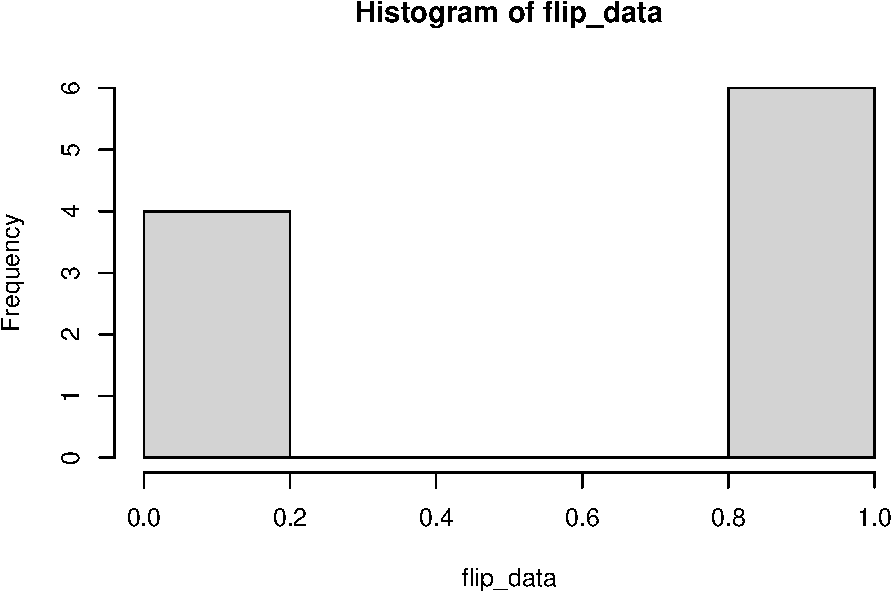
\includegraphics{Bookdown_files/figure-latex/unnamed-chunk-4-1.pdf}

\begin{Shaded}
\begin{Highlighting}[]
                        \CommentTok{\# this prettier with ggplot2, but we don\textquotesingle{}t need that right}
                        \CommentTok{\# now.}
\end{Highlighting}
\end{Shaded}

\hypertarget{why-doesnt-ols-work-for-binomial-data}{%
\section{Why doesn't OLS work for Binomial Data?}\label{why-doesnt-ols-work-for-binomial-data}}

\hypertarget{link-functions-we-can-use}{%
\section{Link functions we can use}\label{link-functions-we-can-use}}

\hypertarget{ed50}{%
\section{ED50}\label{ed50}}

\hypertarget{poisson-regression}{%
\chapter{Poisson Regression}\label{poisson-regression}}

\hypertarget{what-is-poisson-data}{%
\section{What is Poisson data?}\label{what-is-poisson-data}}

Poisson data occurs when there is a need to model counts. The counts of events being modeled should be independent and the upper limit of the counts is much greater than the majority of the counts or even may not exist. Possion GLMs can also be used to model rates, used to compare counts across the unit of populations, when a Binomial GLM would not be appropriate. This occurs when populations are large and the rate of occurance is very small, usually less than 1\%. The Poisson distribution has probability function P(y\textbar{}\(\mu\)) = \(e^{-\mu}\mu^y/y!\) for y = 0, 1, 2,\ldots{} and \(\mu\) \textgreater{} 0.

\hypertarget{why-ordinary-least-squares-does-not-work-for-poisson-data}{%
\section{Why ordinary least squares does not work for Poisson data}\label{why-ordinary-least-squares-does-not-work-for-poisson-data}}

Ordinary least squares (OLS) regression cannot be used for Poisson data. Count data violates the constant variance assumption of OLS because as the counts are smaller and approach 0, the variance of the response must decrease, and as the counts grow larger, the variance of the response will tend to increase. The normal distribution is also not adequate for modeling the random component of count data because counts are both non-negative and discrete. The Poisson distribution is a more suitable option to model count data.

\hypertarget{link-functions-for-poisson-glms}{%
\section{Link functions for Poisson GLM's}\label{link-functions-for-poisson-glms}}

The most common link function used for Poisson regression is the logrithmic link function because it guarentees that \(\mu\) will be greater than 0 and makes interpretation of the regression parameters more straightforward, since they are interpreted as having multiplicative effects. The systematic component of a Poisson GLM is \(\mu = e^{\beta_0 + \beta_1x_1 + ... + \beta_px_p}\) and increasing \(x_j\) by one will increase \(\mu\) by a factor of \(\beta_j\). Other link functions, while less commmon, can be used for a Poisson GLM. The identity link function, where \(\eta = \mu\), or the sqrt link function, where \(\eta = \sqrt{\mu}\), are two options. When all of the explanatory variables are quantitative, the data are modeled by a Poisson regression model. Additionally, quantile residuals should be used to asses the model fit since the data are discrete. Count data can also be represented in contingency tables so that observations can be cross-classified in their relevant categories. These data are modeled using a log-linear model, where all of the explanatory variables are qualitative.

\hypertarget{problems-of-overdispersion-and-solutions}{%
\section{Problems of overdispersion and solutions}\label{problems-of-overdispersion-and-solutions}}

A characteristic of the Poisson distribution is that the mean \(\mu\) equals the variance. However, when modeling real data, this assumption can be a bit \({fishy}\), since the variance is usually greater than \(\mu\), which is overdispersion. Overdispersion occurs because the events being counted have a positive correlation and so are not independent. Overdispersion is an issue in Poisson GLM's because the standard errors of the estimated \(\beta_j\) will be underestimated, making the model's explanatory variables appear more significant than they actually are. Models fit using the Poisson family can be checked for overdispersion by comparing the residual deviance compared to the residual degrees of freedom. If the residual deviance is greater than the degrees of freedom, the model is overdispersed, and if the residual deviance is much less than the degrees of freedom, the model is underdispersed, a less frequent occurence. A large residual deviance compared to the residual degrees of freedom could also indicate a lack of fit, but this can be checked by eliminating outliers and fits the a model with the most explanatory variables possible. The residual deviance will still be large if overdispersion is the issue. Similarly, the Pearson goodness-of-fit statistic can be compared to the residual degrees of freedom to check for overdispersion. This method should be used when the counts are small, so asymptotic approximations would not be appropriate. Here, large goodness-of-fit statistics indicate a poor fit. If there is overdispersion after fitting a Poisson GLM, the model can be fit using other related families. By modeling the data using a hierarchical model to add more variability, \(\mu\) can be treated as a random variable, resulting in the response variable of interest following a negative binomial distribution. The expectation of \(y_i\) is \(\mu_i\) and the variance of \(y_i\) is now \(\mu_i + \psi\mu_i^2\), where \(\psi\mu_i^2\) is the added overdispersion term and \(\psi\) is larger when overdispersion is greater. The MASS package contains the function glm.nb() to model negative binomial GLMs. The standard link function is the log-link function so that \(\mu\) \textgreater{} 0, and similar to the Poisson GLM, quantile residuals should be used. Quasi-Poisson models are another alternative to Poisson GLMs when there is overdispersion. The variance of \(y_i\) is now \(\phi\mu_i\), where \(\phi\) \textgreater{} 1 represents overdispersion and raises standard errors to a factor of \(\sqrt{\phi}\). Quasi-Poisson models can be fit in R by family = quasipoisson(). Quantile residuals cannot be found because the quasi-Poisson model is not a probability model but standardized deviance residuals can be examoned.

\hypertarget{learnr-test}{%
\chapter{LearnR test}\label{learnr-test}}

Here is an embedded learnR tutorial from a published shiny app.

\begin{Shaded}
\begin{Highlighting}[]
\NormalTok{knitr}\OperatorTok{::}\KeywordTok{include\_url}\NormalTok{(}\StringTok{"https://emilypalmer.shinyapps.io/GRM\_LearnR/"}\NormalTok{, }
  \DataTypeTok{height =} \StringTok{"600px"}\NormalTok{)}
\end{Highlighting}
\end{Shaded}


  \bibliography{book.bib,packages.bib}

\end{document}
